% Options for packages loaded elsewhere
\PassOptionsToPackage{unicode}{hyperref}
\PassOptionsToPackage{hyphens}{url}
%
\documentclass[
]{article}
\usepackage{lmodern}
\usepackage{amsmath}
\usepackage{ifxetex,ifluatex}
\ifnum 0\ifxetex 1\fi\ifluatex 1\fi=0 % if pdftex
  \usepackage[T1]{fontenc}
  \usepackage[utf8]{inputenc}
  \usepackage{textcomp} % provide euro and other symbols
  \usepackage{amssymb}
\else % if luatex or xetex
  \usepackage{unicode-math}
  \defaultfontfeatures{Scale=MatchLowercase}
  \defaultfontfeatures[\rmfamily]{Ligatures=TeX,Scale=1}
\fi
% Use upquote if available, for straight quotes in verbatim environments
\IfFileExists{upquote.sty}{\usepackage{upquote}}{}
\IfFileExists{microtype.sty}{% use microtype if available
  \usepackage[]{microtype}
  \UseMicrotypeSet[protrusion]{basicmath} % disable protrusion for tt fonts
}{}
\makeatletter
\@ifundefined{KOMAClassName}{% if non-KOMA class
  \IfFileExists{parskip.sty}{%
    \usepackage{parskip}
  }{% else
    \setlength{\parindent}{0pt}
    \setlength{\parskip}{6pt plus 2pt minus 1pt}}
}{% if KOMA class
  \KOMAoptions{parskip=half}}
\makeatother
\usepackage{xcolor}
\IfFileExists{xurl.sty}{\usepackage{xurl}}{} % add URL line breaks if available
\IfFileExists{bookmark.sty}{\usepackage{bookmark}}{\usepackage{hyperref}}
\hypersetup{
  pdftitle={Regression Analysis of Baseball Team Performance},
  pdfauthor={Abdellah AitElmouden \textbar{} Gabriel Abreu \textbar{} Jered Ataky \textbar{} Patrick Maloney},
  hidelinks,
  pdfcreator={LaTeX via pandoc}}
\urlstyle{same} % disable monospaced font for URLs
\usepackage[margin=1in]{geometry}
\usepackage{color}
\usepackage{fancyvrb}
\newcommand{\VerbBar}{|}
\newcommand{\VERB}{\Verb[commandchars=\\\{\}]}
\DefineVerbatimEnvironment{Highlighting}{Verbatim}{commandchars=\\\{\}}
% Add ',fontsize=\small' for more characters per line
\usepackage{framed}
\definecolor{shadecolor}{RGB}{248,248,248}
\newenvironment{Shaded}{\begin{snugshade}}{\end{snugshade}}
\newcommand{\AlertTok}[1]{\textcolor[rgb]{0.94,0.16,0.16}{#1}}
\newcommand{\AnnotationTok}[1]{\textcolor[rgb]{0.56,0.35,0.01}{\textbf{\textit{#1}}}}
\newcommand{\AttributeTok}[1]{\textcolor[rgb]{0.77,0.63,0.00}{#1}}
\newcommand{\BaseNTok}[1]{\textcolor[rgb]{0.00,0.00,0.81}{#1}}
\newcommand{\BuiltInTok}[1]{#1}
\newcommand{\CharTok}[1]{\textcolor[rgb]{0.31,0.60,0.02}{#1}}
\newcommand{\CommentTok}[1]{\textcolor[rgb]{0.56,0.35,0.01}{\textit{#1}}}
\newcommand{\CommentVarTok}[1]{\textcolor[rgb]{0.56,0.35,0.01}{\textbf{\textit{#1}}}}
\newcommand{\ConstantTok}[1]{\textcolor[rgb]{0.00,0.00,0.00}{#1}}
\newcommand{\ControlFlowTok}[1]{\textcolor[rgb]{0.13,0.29,0.53}{\textbf{#1}}}
\newcommand{\DataTypeTok}[1]{\textcolor[rgb]{0.13,0.29,0.53}{#1}}
\newcommand{\DecValTok}[1]{\textcolor[rgb]{0.00,0.00,0.81}{#1}}
\newcommand{\DocumentationTok}[1]{\textcolor[rgb]{0.56,0.35,0.01}{\textbf{\textit{#1}}}}
\newcommand{\ErrorTok}[1]{\textcolor[rgb]{0.64,0.00,0.00}{\textbf{#1}}}
\newcommand{\ExtensionTok}[1]{#1}
\newcommand{\FloatTok}[1]{\textcolor[rgb]{0.00,0.00,0.81}{#1}}
\newcommand{\FunctionTok}[1]{\textcolor[rgb]{0.00,0.00,0.00}{#1}}
\newcommand{\ImportTok}[1]{#1}
\newcommand{\InformationTok}[1]{\textcolor[rgb]{0.56,0.35,0.01}{\textbf{\textit{#1}}}}
\newcommand{\KeywordTok}[1]{\textcolor[rgb]{0.13,0.29,0.53}{\textbf{#1}}}
\newcommand{\NormalTok}[1]{#1}
\newcommand{\OperatorTok}[1]{\textcolor[rgb]{0.81,0.36,0.00}{\textbf{#1}}}
\newcommand{\OtherTok}[1]{\textcolor[rgb]{0.56,0.35,0.01}{#1}}
\newcommand{\PreprocessorTok}[1]{\textcolor[rgb]{0.56,0.35,0.01}{\textit{#1}}}
\newcommand{\RegionMarkerTok}[1]{#1}
\newcommand{\SpecialCharTok}[1]{\textcolor[rgb]{0.00,0.00,0.00}{#1}}
\newcommand{\SpecialStringTok}[1]{\textcolor[rgb]{0.31,0.60,0.02}{#1}}
\newcommand{\StringTok}[1]{\textcolor[rgb]{0.31,0.60,0.02}{#1}}
\newcommand{\VariableTok}[1]{\textcolor[rgb]{0.00,0.00,0.00}{#1}}
\newcommand{\VerbatimStringTok}[1]{\textcolor[rgb]{0.31,0.60,0.02}{#1}}
\newcommand{\WarningTok}[1]{\textcolor[rgb]{0.56,0.35,0.01}{\textbf{\textit{#1}}}}
\usepackage{longtable,booktabs}
\usepackage{calc} % for calculating minipage widths
% Correct order of tables after \paragraph or \subparagraph
\usepackage{etoolbox}
\makeatletter
\patchcmd\longtable{\par}{\if@noskipsec\mbox{}\fi\par}{}{}
\makeatother
% Allow footnotes in longtable head/foot
\IfFileExists{footnotehyper.sty}{\usepackage{footnotehyper}}{\usepackage{footnote}}
\makesavenoteenv{longtable}
\usepackage{graphicx}
\makeatletter
\def\maxwidth{\ifdim\Gin@nat@width>\linewidth\linewidth\else\Gin@nat@width\fi}
\def\maxheight{\ifdim\Gin@nat@height>\textheight\textheight\else\Gin@nat@height\fi}
\makeatother
% Scale images if necessary, so that they will not overflow the page
% margins by default, and it is still possible to overwrite the defaults
% using explicit options in \includegraphics[width, height, ...]{}
\setkeys{Gin}{width=\maxwidth,height=\maxheight,keepaspectratio}
% Set default figure placement to htbp
\makeatletter
\def\fps@figure{htbp}
\makeatother
\setlength{\emergencystretch}{3em} % prevent overfull lines
\providecommand{\tightlist}{%
  \setlength{\itemsep}{0pt}\setlength{\parskip}{0pt}}
\setcounter{secnumdepth}{-\maxdimen} % remove section numbering
\usepackage{amsmath}
\usepackage{booktabs}
\usepackage{caption}
\usepackage{longtable}
\ifluatex
  \usepackage{selnolig}  % disable illegal ligatures
\fi

\title{Regression Analysis of Baseball Team Performance}
\author{Abdellah AitElmouden \textbar{} Gabriel Abreu \textbar{} Jered
Ataky \textbar{} Patrick Maloney}
\date{2/12/2021}

\begin{document}
\maketitle

\hypertarget{abstract}{%
\subsection{Abstract}\label{abstract}}

To see how regression will help us evaluate baseball team performance,
this project is designed to explore whether a teams success in any given
season can be predicted or explained by any number of statistics in that
season. Our goal is to build a multiple linear regression model on the
training data to predict the number of wins for the team. we will
explore, analyze and model a historical baseball data set containing
approximately 2200 records. Each record represents a professional
baseball team from the years 1871 to 2006 inclusive, and the data
include the performance of the team for the given year, with all of the
statistics adjusted to match the performance of a 162 game season.

While correlation does not equal causation it is suggested that a focus
on some of the variables such as a focus on either single hits or triple
or more hits to the exclusion of doubles might be worth pursuing. Also
the data suggests that a focus on home runs allowed may not be worth
giving up a number of more normal hits.

\ldots..To add more here\ldots.

\hypertarget{introduction}{%
\subsection{Introduction}\label{introduction}}

Because baseball is so numbers-heavy, there are many different
statistics to consider when searching for the best predictors of team
success. There are offensive statistics (offense meaning when a team is
batting) and defensive statistics (defense meaning when a team is in the
field). These categories can be broken up into many more subcategories.
However, for the purpose of the this project we will use the available
data to build a multiple linear regression model on the training data to
predict the number of wins for the team.

To see how regression will help us predict the number of wins for the
team, we actually don't need to understand all the details about the
game of baseball, which has over 100 rules. Here, we distill the sport
to the basic knowledge one needs to know how to effectively attack the
data science problem. The goal of a baseball game is to score more runs
(points) than the other team. Each team has 9 batters that have an
opportunity to hit a ball with a bat in a predetermined order. After the
9th batter has had their turn, the first batter bats again, then the
second, and so on. Each time a batter has an opportunity to bat, we call
it a plate appearance (PA). At each PA, the other team's pitcher throws
the ball and the batter tries to hit it. The PA ends with an binary
outcome: the batter either makes an out (failure) and returns to the
bench or the batter doesn't (success) and can run around the bases, and
potentially score a run (reach all 4 bases). Each team gets nine tries,
referred to as innings, to score runs and each inning ends after three
outs (three failures).

\newpage

\hypertarget{data-exploration}{%
\subsection{Data Exploration}\label{data-exploration}}

The dataset we will be using was provided in csv file. The files contain
approximately 2200 records. Each record represents a professional
baseball team from the years 1871 to 2006 inclusive. Each record has the
performance of the team for the given year, with all of the statistics
adjusted to match the performance of a 162 game season. The game
statistics that will be used in this study are the following:

\begin{longtable}[]{@{}lll@{}}
\toprule
\begin{minipage}[b]{(\columnwidth - 2\tabcolsep) * \real{0.22}}\raggedright
VARIABLE NAME\strut
\end{minipage} &
\begin{minipage}[b]{(\columnwidth - 2\tabcolsep) * \real{0.48}}\raggedright
DEFINITION\strut
\end{minipage} &
\begin{minipage}[b]{(\columnwidth - 2\tabcolsep) * \real{0.30}}\raggedright
THEORETICAL EFFECT\strut
\end{minipage}\tabularnewline
\midrule
\endhead
\begin{minipage}[t]{(\columnwidth - 2\tabcolsep) * \real{0.22}}\raggedright
INDEX\strut
\end{minipage} &
\begin{minipage}[t]{(\columnwidth - 2\tabcolsep) * \real{0.48}}\raggedright
Identification Variable (do not use)\strut
\end{minipage} &
\begin{minipage}[t]{(\columnwidth - 2\tabcolsep) * \real{0.30}}\raggedright
None\strut
\end{minipage}\tabularnewline
\begin{minipage}[t]{(\columnwidth - 2\tabcolsep) * \real{0.22}}\raggedright
TARGET\_WINS\strut
\end{minipage} &
\begin{minipage}[t]{(\columnwidth - 2\tabcolsep) * \real{0.48}}\raggedright
Number of wins\strut
\end{minipage} &
\begin{minipage}[t]{(\columnwidth - 2\tabcolsep) * \real{0.30}}\raggedright
Outcome Variable\strut
\end{minipage}\tabularnewline
\begin{minipage}[t]{(\columnwidth - 2\tabcolsep) * \real{0.22}}\raggedright
TEAM\_BATTING\_H\strut
\end{minipage} &
\begin{minipage}[t]{(\columnwidth - 2\tabcolsep) * \real{0.48}}\raggedright
Base Hits by batters (1B,2B,3B,HR)\strut
\end{minipage} &
\begin{minipage}[t]{(\columnwidth - 2\tabcolsep) * \real{0.30}}\raggedright
Positive Impact on Wins\strut
\end{minipage}\tabularnewline
\begin{minipage}[t]{(\columnwidth - 2\tabcolsep) * \real{0.22}}\raggedright
TEAM\_BATTING\_2B\strut
\end{minipage} &
\begin{minipage}[t]{(\columnwidth - 2\tabcolsep) * \real{0.48}}\raggedright
Doubles by batters (2B)\strut
\end{minipage} &
\begin{minipage}[t]{(\columnwidth - 2\tabcolsep) * \real{0.30}}\raggedright
Positive Impact on Wins\strut
\end{minipage}\tabularnewline
\begin{minipage}[t]{(\columnwidth - 2\tabcolsep) * \real{0.22}}\raggedright
TEAM\_BATTING\_3B\strut
\end{minipage} &
\begin{minipage}[t]{(\columnwidth - 2\tabcolsep) * \real{0.48}}\raggedright
Triples by batters (3B)\strut
\end{minipage} &
\begin{minipage}[t]{(\columnwidth - 2\tabcolsep) * \real{0.30}}\raggedright
Positive Impact on Wins\strut
\end{minipage}\tabularnewline
\begin{minipage}[t]{(\columnwidth - 2\tabcolsep) * \real{0.22}}\raggedright
TEAM\_BATTING\_HR\strut
\end{minipage} &
\begin{minipage}[t]{(\columnwidth - 2\tabcolsep) * \real{0.48}}\raggedright
Homeruns by batters (4B)\strut
\end{minipage} &
\begin{minipage}[t]{(\columnwidth - 2\tabcolsep) * \real{0.30}}\raggedright
Positive Impact on Wins\strut
\end{minipage}\tabularnewline
\begin{minipage}[t]{(\columnwidth - 2\tabcolsep) * \real{0.22}}\raggedright
TEAM\_BATTING\_BB\strut
\end{minipage} &
\begin{minipage}[t]{(\columnwidth - 2\tabcolsep) * \real{0.48}}\raggedright
Walks by batters\strut
\end{minipage} &
\begin{minipage}[t]{(\columnwidth - 2\tabcolsep) * \real{0.30}}\raggedright
Positive Impact on Wins\strut
\end{minipage}\tabularnewline
\begin{minipage}[t]{(\columnwidth - 2\tabcolsep) * \real{0.22}}\raggedright
TEAM\_BATTING\_HBP\strut
\end{minipage} &
\begin{minipage}[t]{(\columnwidth - 2\tabcolsep) * \real{0.48}}\raggedright
Batters hit by pitch (get a free base)\strut
\end{minipage} &
\begin{minipage}[t]{(\columnwidth - 2\tabcolsep) * \real{0.30}}\raggedright
Positive Impact on Wins\strut
\end{minipage}\tabularnewline
\begin{minipage}[t]{(\columnwidth - 2\tabcolsep) * \real{0.22}}\raggedright
TEAM\_BATTING\_SO\strut
\end{minipage} &
\begin{minipage}[t]{(\columnwidth - 2\tabcolsep) * \real{0.48}}\raggedright
Strikeouts by batters\strut
\end{minipage} &
\begin{minipage}[t]{(\columnwidth - 2\tabcolsep) * \real{0.30}}\raggedright
Negative Impact on Wins\strut
\end{minipage}\tabularnewline
\begin{minipage}[t]{(\columnwidth - 2\tabcolsep) * \real{0.22}}\raggedright
TEAM\_BASERUN\_SB\strut
\end{minipage} &
\begin{minipage}[t]{(\columnwidth - 2\tabcolsep) * \real{0.48}}\raggedright
Stolen bases\strut
\end{minipage} &
\begin{minipage}[t]{(\columnwidth - 2\tabcolsep) * \real{0.30}}\raggedright
Positive Impact on Wins\strut
\end{minipage}\tabularnewline
\begin{minipage}[t]{(\columnwidth - 2\tabcolsep) * \real{0.22}}\raggedright
TEAM\_BASERUN\_CS\strut
\end{minipage} &
\begin{minipage}[t]{(\columnwidth - 2\tabcolsep) * \real{0.48}}\raggedright
Caught stealing\strut
\end{minipage} &
\begin{minipage}[t]{(\columnwidth - 2\tabcolsep) * \real{0.30}}\raggedright
Negative Impact on Wins\strut
\end{minipage}\tabularnewline
\begin{minipage}[t]{(\columnwidth - 2\tabcolsep) * \real{0.22}}\raggedright
TEAM\_FIELDING\_E\strut
\end{minipage} &
\begin{minipage}[t]{(\columnwidth - 2\tabcolsep) * \real{0.48}}\raggedright
Errors\strut
\end{minipage} &
\begin{minipage}[t]{(\columnwidth - 2\tabcolsep) * \real{0.30}}\raggedright
Negative Impact on Wins\strut
\end{minipage}\tabularnewline
\begin{minipage}[t]{(\columnwidth - 2\tabcolsep) * \real{0.22}}\raggedright
TEAM\_FIELDING\_DP\strut
\end{minipage} &
\begin{minipage}[t]{(\columnwidth - 2\tabcolsep) * \real{0.48}}\raggedright
Double Plays\strut
\end{minipage} &
\begin{minipage}[t]{(\columnwidth - 2\tabcolsep) * \real{0.30}}\raggedright
Positive Impact on Wins\strut
\end{minipage}\tabularnewline
\begin{minipage}[t]{(\columnwidth - 2\tabcolsep) * \real{0.22}}\raggedright
TEAM\_PITCHING\_BB\strut
\end{minipage} &
\begin{minipage}[t]{(\columnwidth - 2\tabcolsep) * \real{0.48}}\raggedright
Walks allowed\strut
\end{minipage} &
\begin{minipage}[t]{(\columnwidth - 2\tabcolsep) * \real{0.30}}\raggedright
Negative Impact on Wins\strut
\end{minipage}\tabularnewline
\begin{minipage}[t]{(\columnwidth - 2\tabcolsep) * \real{0.22}}\raggedright
TEAM\_PITCHING\_H\strut
\end{minipage} &
\begin{minipage}[t]{(\columnwidth - 2\tabcolsep) * \real{0.48}}\raggedright
Hits allowed\strut
\end{minipage} &
\begin{minipage}[t]{(\columnwidth - 2\tabcolsep) * \real{0.30}}\raggedright
Negative Impact on Wins\strut
\end{minipage}\tabularnewline
\begin{minipage}[t]{(\columnwidth - 2\tabcolsep) * \real{0.22}}\raggedright
TEAM\_PITCHING\_HR\strut
\end{minipage} &
\begin{minipage}[t]{(\columnwidth - 2\tabcolsep) * \real{0.48}}\raggedright
Homeruns allowed\strut
\end{minipage} &
\begin{minipage}[t]{(\columnwidth - 2\tabcolsep) * \real{0.30}}\raggedright
Negative Impact on Wins\strut
\end{minipage}\tabularnewline
\begin{minipage}[t]{(\columnwidth - 2\tabcolsep) * \real{0.22}}\raggedright
TEAM\_PITCHING\_SO\strut
\end{minipage} &
\begin{minipage}[t]{(\columnwidth - 2\tabcolsep) * \real{0.48}}\raggedright
Strikeouts by pitchers\strut
\end{minipage} &
\begin{minipage}[t]{(\columnwidth - 2\tabcolsep) * \real{0.30}}\raggedright
Positive Impact on Wins\strut
\end{minipage}\tabularnewline
\bottomrule
\end{longtable}

The initial steps are to download the data and take a quick glimpse of
the columns, their data types, number of columns, and rows. Based on
initial observations, the data contains 2276 teams with a variety of
baseball performance statistics.

\begin{verbatim}
## Rows: 2,276
## Columns: 17
## $ INDEX            <int> 1, 2, 3, 4, 5, 6, 7, 8, 11, 12, 13, 15, 16, 17, 18...
## $ TARGET_WINS      <int> 39, 70, 86, 70, 82, 75, 80, 85, 86, 76, 78, 68, 72...
## $ TEAM_BATTING_H   <int> 1445, 1339, 1377, 1387, 1297, 1279, 1244, 1273, 13...
## $ TEAM_BATTING_2B  <int> 194, 219, 232, 209, 186, 200, 179, 171, 197, 213, ...
## $ TEAM_BATTING_3B  <int> 39, 22, 35, 38, 27, 36, 54, 37, 40, 18, 27, 31, 41...
## $ TEAM_BATTING_HR  <int> 13, 190, 137, 96, 102, 92, 122, 115, 114, 96, 82, ...
## $ TEAM_BATTING_BB  <int> 143, 685, 602, 451, 472, 443, 525, 456, 447, 441, ...
## $ TEAM_BATTING_SO  <int> 842, 1075, 917, 922, 920, 973, 1062, 1027, 922, 82...
## $ TEAM_BASERUN_SB  <int> NA, 37, 46, 43, 49, 107, 80, 40, 69, 72, 60, 119, ...
## $ TEAM_BASERUN_CS  <int> NA, 28, 27, 30, 39, 59, 54, 36, 27, 34, 39, 79, 10...
## $ TEAM_BATTING_HBP <int> NA, NA, NA, NA, NA, NA, NA, NA, NA, NA, NA, NA, NA...
## $ TEAM_PITCHING_H  <int> 9364, 1347, 1377, 1396, 1297, 1279, 1244, 1281, 13...
## $ TEAM_PITCHING_HR <int> 84, 191, 137, 97, 102, 92, 122, 116, 114, 96, 86, ...
## $ TEAM_PITCHING_BB <int> 927, 689, 602, 454, 472, 443, 525, 459, 447, 441, ...
## $ TEAM_PITCHING_SO <int> 5456, 1082, 917, 928, 920, 973, 1062, 1033, 922, 8...
## $ TEAM_FIELDING_E  <int> 1011, 193, 175, 164, 138, 123, 136, 112, 127, 131,...
## $ TEAM_FIELDING_DP <int> NA, 155, 153, 156, 168, 149, 186, 136, 169, 159, 1...
\end{verbatim}

\newpage

At first glance, the column BATTING\_HBP has numerous NA values that
will need to be addressed before building a model. Figure 1 show summary
statistics of the target wins. The noteworthy statistics are the average
number of wins in a season is 81 games, the median number of wins in a
season is 82 games, and the standard deviation is 16 games.

\begin{center}
Figure 1 :  Summary Statistics
\end{center}

\begin{longtable}[]{@{}ll@{}}
\toprule
\textbf{Characteristic} & \textbf{N = 2,276}\tabularnewline
\midrule
\endhead
TARGET\_WINS & 81 (16) 82 0 146\tabularnewline
TEAM\_BATTING\_H & 1,469 (145) 1,454 891 2,554\tabularnewline
TEAM\_BATTING\_2B & 241 (47) 238 69 458\tabularnewline
TEAM\_BATTING\_3B & 55 (28) 47 0 223\tabularnewline
TEAM\_BATTING\_HR & 100 (61) 102 0 264\tabularnewline
TEAM\_BATTING\_BB & 502 (123) 512 0 878\tabularnewline
TEAM\_BATTING\_HBP & 59 (13) 58 29 95\tabularnewline
TEAM\_BATTING\_SO & 736 (249) 750 0 1,399\tabularnewline
TEAM\_BASERUN\_SB & 125 (88) 101 0 697\tabularnewline
TEAM\_BASERUN\_CS & 53 (23) 49 0 201\tabularnewline
TEAM\_FIELDING\_E & 246 (228) 159 65 1,898\tabularnewline
TEAM\_FIELDING\_DP & 146 (26) 149 52 228\tabularnewline
TEAM\_PITCHING\_BB & 553 (166) 536 0 3,645\tabularnewline
TEAM\_PITCHING\_SO & 818 (553) 814 0 19,278\tabularnewline
\bottomrule
\end{longtable}

In recent years in baseball, slugging percentage has become a popular
statistic in the analytics department of many teams. The name is a
misnomer, since it is not actually a percentage, but rather a measure of
bases produced per at bat, and is calculated by total bases (i.e.~1 for
a single, 4 for a HR) divided by total at-bats. However, since this
dataset doesn't contain information on at-bats, we will use a modified
version of slugging percentage that measures average bases produced per
hit.

\begin{Shaded}
\begin{Highlighting}[]
\NormalTok{singles }\OtherTok{\textless{}{-}}\NormalTok{ train\_data}\SpecialCharTok{$}\NormalTok{TEAM\_BATTING\_H }\SpecialCharTok{{-}}\NormalTok{ (train\_data}\SpecialCharTok{$}\NormalTok{TEAM\_BATTING\_2B }\SpecialCharTok{+}\NormalTok{ train\_data}\SpecialCharTok{$}\NormalTok{TEAM\_BATTING\_3B }\SpecialCharTok{+}\NormalTok{ train\_data}\SpecialCharTok{$}\NormalTok{TEAM\_BATTING\_HR)}

\NormalTok{train\_data}\SpecialCharTok{$}\NormalTok{TEAM\_BATTING\_SLG }\OtherTok{\textless{}{-}}\NormalTok{ ((train\_data}\SpecialCharTok{$}\NormalTok{TEAM\_BATTING\_HR }\SpecialCharTok{*}\DecValTok{4}\NormalTok{)}\SpecialCharTok{+}\NormalTok{ (train\_data}\SpecialCharTok{$}\NormalTok{TEAM\_BATTING\_3B}\SpecialCharTok{*}\DecValTok{3}\NormalTok{) }\SpecialCharTok{+}\NormalTok{ (train\_data}\SpecialCharTok{$}\NormalTok{TEAM\_BATTING\_2B}\SpecialCharTok{*}\DecValTok{2}\NormalTok{)}\SpecialCharTok{+}\NormalTok{ singles)}\SpecialCharTok{/}\NormalTok{train\_data}\SpecialCharTok{$}\NormalTok{TEAM\_BATTING\_H}
\end{Highlighting}
\end{Shaded}

\begin{center}
Mean (SD) Median Minimum Maximum 
\end{center}

By examining the target wins variable in detail, there is a clear
guideline of how many wins each team should approximately win. Most
teams will likely win the average number of games (81), but there will
be some variability from the average with some teams winning more or
less than 81 games.

The other variables also play an important role in understanding the
data. In Figure 1, summary statistics are presented for all the
variables. it is sufficient in getting the gist of each variable's
distribution. For example, the average Base Hits by batters per team is
1469 with the minimum base hits at 891 and maximum base hits at 2554.
Remember that the dataset contains baseball statistics on 2276 teams.
Missing values were excluded from the summary and they will be dealt
with in the data preparation section of this report.

A quick look at Figure 2 will reveal the distribution of the target
wins. The distribution is approximately normal with a majority of the
target wins falling in the center of the distribution.The approximate
normal distribution is confirmed by the QQ plot below the distribution
plot. Most of the target wins fall on the line in the QQ plot with some
data points diverging at the ends. This indicates possibility of
outliers where some teams are winning more games or losing more games
than what is expected in the normal range.In the boxplot, there are
points that fall outside the whiskers which confirms our suspicions of
outliers seen in the QQ plot.

\includegraphics{Assignment1_files/figure-latex/unnamed-chunk-4-1.pdf}

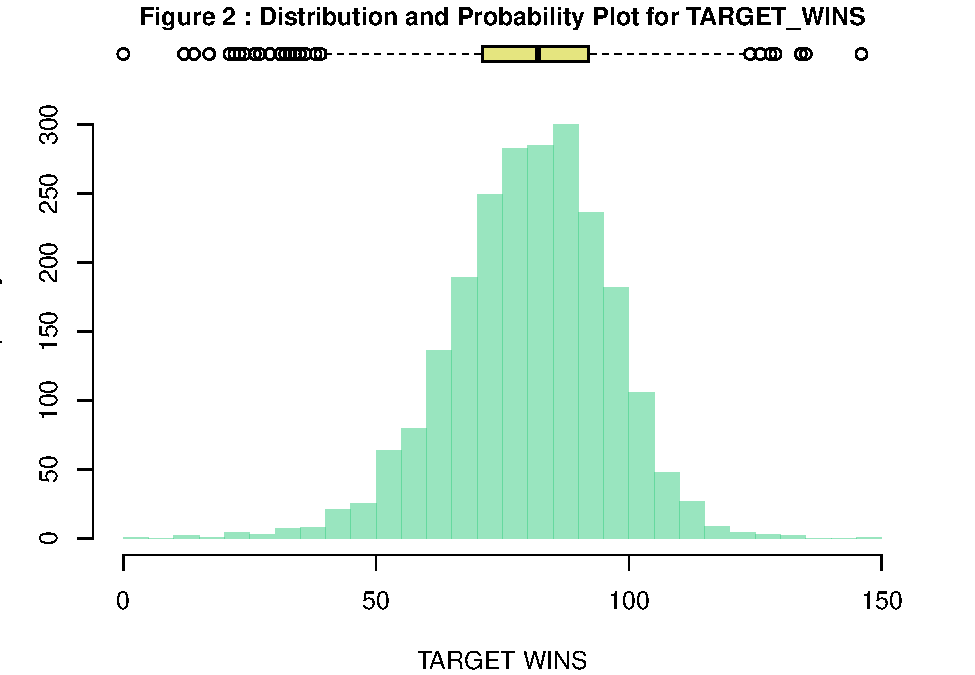
\includegraphics{Assignment1_files/figure-latex/unnamed-chunk-5-1.pdf}

Now in order to build our models properly It's worth exploring for other
columns with NA values.

\captionsetup[table]{labelformat=empty,skip=1pt}
\begin{longtable}{lr}
\toprule
Columns\_w\_NA & Percent\_NA \\ 
\midrule
team\_batting\_so & 4.481547 \\ 
team\_baserun\_sb & 5.755712 \\ 
team\_baserun\_cs & 33.919156 \\ 
team\_batting\_hbp & 91.608084 \\ 
team\_pitching\_so & 4.481547 \\ 
team\_fielding\_dp & 12.565905 \\ 
\bottomrule
\end{longtable}

\begin{Shaded}
\begin{Highlighting}[]
\CommentTok{\#train\_data[{-}c(1)] \%\textgreater{}\%}
\CommentTok{\#  gather() \%\textgreater{}\% }
\CommentTok{\#  ggplot(aes(value)) +}
\CommentTok{\#    facet\_wrap(\textasciitilde{} key, scales = "free") +}
\CommentTok{\#    geom\_histogram(binwidth=1)}
\end{Highlighting}
\end{Shaded}

\hypertarget{outliers}{%
\subsubsection{Outliers}\label{outliers}}

The following diagram shows the outliers for all the variables, both
dependent and independent.

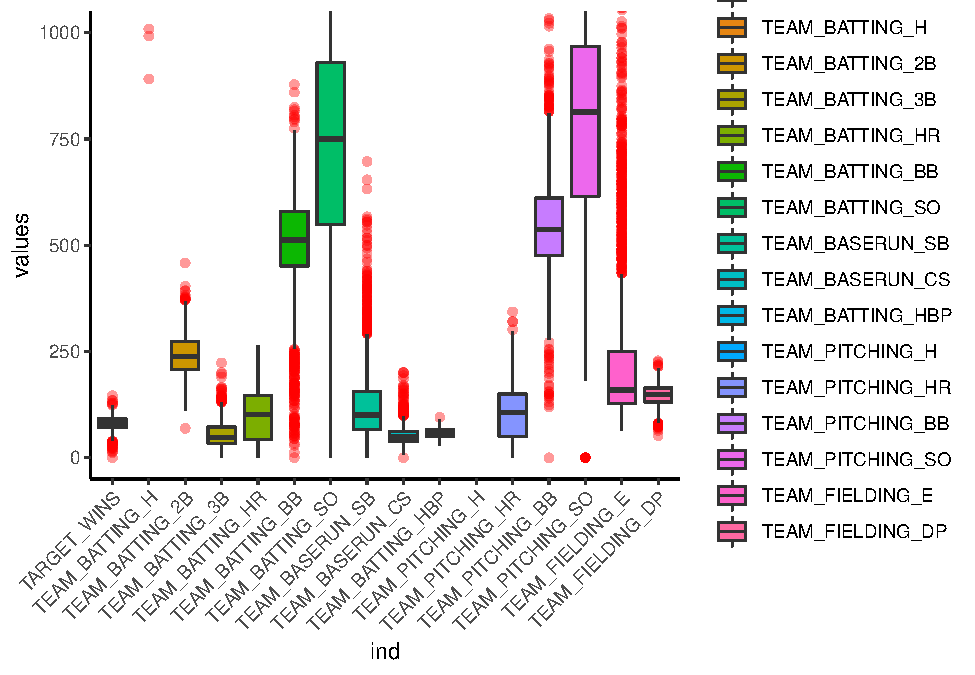
\includegraphics{Assignment1_files/figure-latex/unnamed-chunk-8-1.pdf}
As we can see from the graph only 4 of the 16 variables are normally or
close to normally distributed. the other 12 variables have a significant
skew. The response variable Target\_wins seems to be normally
distributed. Batting\_Hr, Batting\_SO and Pitching\_HR are bi-modal. 10
of the 16 variables have a minimum value of 0. This is not a major
concern as the total \% of 0 in each column is less than 1\%. The
variables Batting\_BB, Batting\_CS, Baserun\_SB, Pitching\_BB and
Fielding\_E have a significant number of outliers.

\hypertarget{correlations-among-predictors-and-variable-selection}{%
\subsubsection{Correlations among predictors and Variable
Selection}\label{correlations-among-predictors-and-variable-selection}}

It is possible that not all variables will need to be used in creating
an accurate model. In Figure 4, a correlation value is computed for each
variable against target wins. Some variables are highly correlated with
target wins, while other variables are not. For example, Base Hits by
batters has a value of 0.38877 which is high while Caught stealing is
barely correlated with target wins with a value of 0.0224.There is also
a column for p-values which indicates whether the correlations are
significant. We can use a decision rule of 95\% meaning any variable
with a p-value of less than 0.05 is significant. It appears that
Strikeouts by batters (TEAM\_BATTING\_SO),Caught
stealing(TEAM\_BASERUN\_CS), Batters hit by pitch (TEAM\_BATTING\_HBP),
and Double plays (TEAM\_FIELDING\_DP)do not meet our decision rule and
could be excluded from use.

\captionsetup[table]{labelformat=empty,skip=1pt}
\begin{longtable}{lr}
\toprule
term & TARGET\_WINS \\ 
\midrule
INDEX & -0.02105643 \\ 
TEAM\_BATTING\_H & 0.38876752 \\ 
TEAM\_BATTING\_2B & 0.28910365 \\ 
TEAM\_BATTING\_3B & 0.14260841 \\ 
TEAM\_BATTING\_HR & 0.17615320 \\ 
TEAM\_BATTING\_BB & 0.23255986 \\ 
TEAM\_BATTING\_SO & -0.03175071 \\ 
TEAM\_BASERUN\_SB & 0.13513892 \\ 
TEAM\_BASERUN\_CS & 0.02240407 \\ 
TEAM\_BATTING\_HBP & 0.07350424 \\ 
TEAM\_PITCHING\_H & -0.10993705 \\ 
TEAM\_PITCHING\_HR & 0.18901373 \\ 
TEAM\_PITCHING\_BB & 0.12417454 \\ 
TEAM\_PITCHING\_SO & -0.07843609 \\ 
TEAM\_FIELDING\_E & -0.17648476 \\ 
TEAM\_FIELDING\_DP & -0.03485058 \\ 
TEAM\_BATTING\_SLG & 0.19052019 \\ 
\bottomrule
\end{longtable}

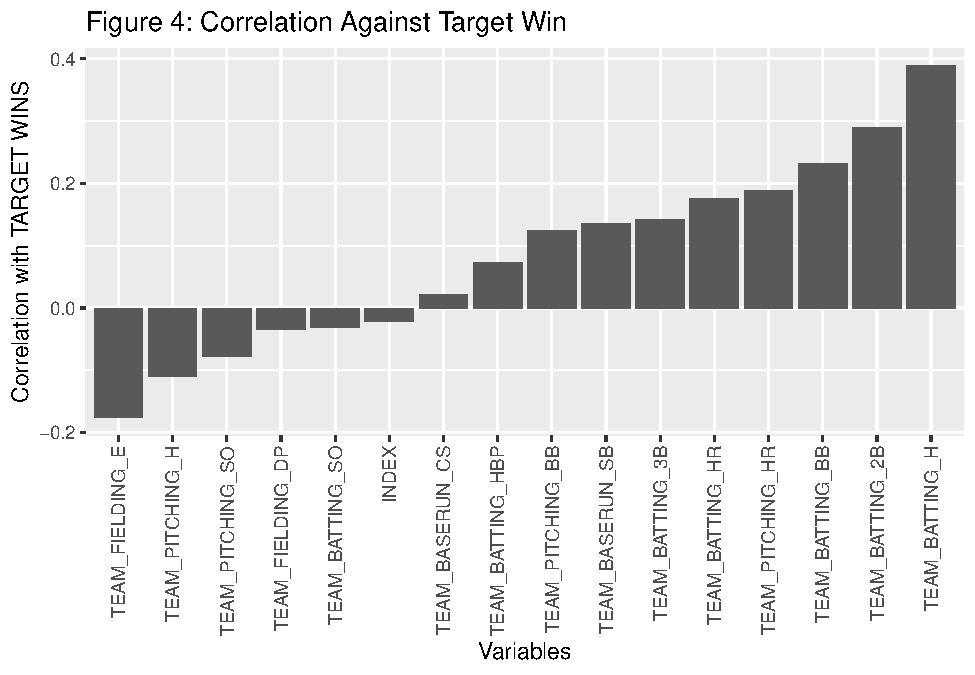
\includegraphics{Assignment1_files/figure-latex/unnamed-chunk-10-1.pdf}
Before entirely excluding variables, it is a good idea to transform the
data by fixing missing values or combining variables and reexamine the
viability of those variables for predicting wins.

\begin{Shaded}
\begin{Highlighting}[]
\CommentTok{\#pairwise.complete.obs ignores NA values and computes correlation on complete observations}
\CommentTok{\#we might have to run these corrplots again after we handle the NA values}
\FunctionTok{chart.Correlation}\NormalTok{(train\_data[}\SpecialCharTok{{-}}\FunctionTok{c}\NormalTok{(}\DecValTok{1}\NormalTok{)], }\AttributeTok{histograme=}\ConstantTok{TRUE}\NormalTok{, }\AttributeTok{method=} \StringTok{"pearson"}\NormalTok{, }\AttributeTok{use=}\StringTok{"pairwise.complete.obs"}\NormalTok{)}
\end{Highlighting}
\end{Shaded}

\includegraphics{Assignment1_files/figure-latex/unnamed-chunk-11-1.pdf}

\begin{Shaded}
\begin{Highlighting}[]
\NormalTok{data.corr }\OtherTok{\textless{}{-}} \FunctionTok{cor}\NormalTok{(train\_data[}\SpecialCharTok{{-}}\FunctionTok{c}\NormalTok{(}\DecValTok{1}\NormalTok{)], }\AttributeTok{use=}\StringTok{"pairwise.complete.obs"}\NormalTok{)}

\FunctionTok{corrplot}\NormalTok{(data.corr, }\AttributeTok{type =} \StringTok{"lower"}\NormalTok{, }\AttributeTok{method=}\StringTok{"square"}\NormalTok{)}
\end{Highlighting}
\end{Shaded}

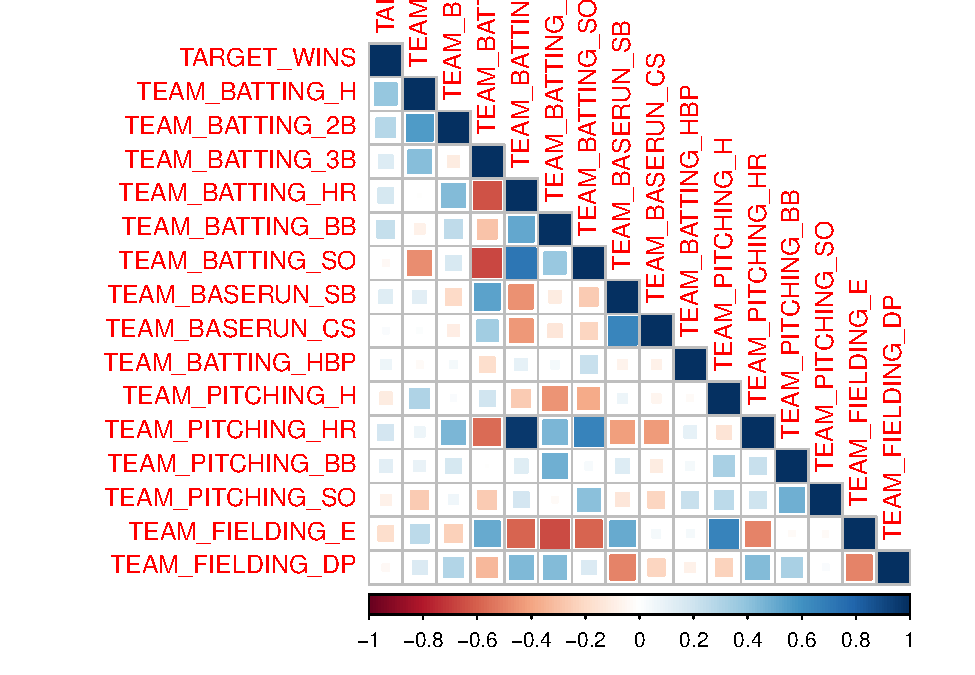
\includegraphics{Assignment1_files/figure-latex/unnamed-chunk-12-1.pdf}

\begin{Shaded}
\begin{Highlighting}[]
\CommentTok{\#eliminate INDEX from data frame}
\NormalTok{data\_no\_index }\OtherTok{\textless{}{-}}\NormalTok{ train\_data[}\SpecialCharTok{{-}}\FunctionTok{c}\NormalTok{(}\DecValTok{1}\NormalTok{)]}

\NormalTok{cor\_matrix }\OtherTok{\textless{}{-}} \FunctionTok{rcorr}\NormalTok{(}\FunctionTok{as.matrix}\NormalTok{(data\_no\_index))}

\FunctionTok{flattenCorrMatrix}\NormalTok{(cor\_matrix}\SpecialCharTok{$}\NormalTok{r, cor\_matrix}\SpecialCharTok{$}\NormalTok{P)}
\end{Highlighting}
\end{Shaded}

\begin{verbatim}
##                  row           column          cor            p
## 1        TARGET_WINS   TEAM_BATTING_H  0.388767521 0.000000e+00
## 2        TARGET_WINS  TEAM_BATTING_2B  0.289103645 0.000000e+00
## 3     TEAM_BATTING_H  TEAM_BATTING_2B  0.562849678 0.000000e+00
## 4        TARGET_WINS  TEAM_BATTING_3B  0.142608411 8.217427e-12
## 5     TEAM_BATTING_H  TEAM_BATTING_3B  0.427696575 0.000000e+00
## 6    TEAM_BATTING_2B  TEAM_BATTING_3B -0.107305824 2.877545e-07
## 7        TARGET_WINS  TEAM_BATTING_HR  0.176153200 0.000000e+00
## 8     TEAM_BATTING_H  TEAM_BATTING_HR -0.006544685 7.549934e-01
## 9    TEAM_BATTING_2B  TEAM_BATTING_HR  0.435397293 0.000000e+00
## 10   TEAM_BATTING_3B  TEAM_BATTING_HR -0.635566946 0.000000e+00
## 11       TARGET_WINS  TEAM_BATTING_BB  0.232559864 0.000000e+00
## 12    TEAM_BATTING_H  TEAM_BATTING_BB -0.072464013 5.407324e-04
## 13   TEAM_BATTING_2B  TEAM_BATTING_BB  0.255726103 0.000000e+00
## 14   TEAM_BATTING_3B  TEAM_BATTING_BB -0.287235841 0.000000e+00
## 15   TEAM_BATTING_HR  TEAM_BATTING_BB  0.513734810 0.000000e+00
## 16       TARGET_WINS  TEAM_BATTING_SO -0.031750708 1.388904e-01
## 17    TEAM_BATTING_H  TEAM_BATTING_SO -0.463853571 0.000000e+00
## 18   TEAM_BATTING_2B  TEAM_BATTING_SO  0.162685188 2.309264e-14
## 19   TEAM_BATTING_3B  TEAM_BATTING_SO -0.669781188 0.000000e+00
## 20   TEAM_BATTING_HR  TEAM_BATTING_SO  0.727069348 0.000000e+00
## 21   TEAM_BATTING_BB  TEAM_BATTING_SO  0.379750866 0.000000e+00
## 22       TARGET_WINS  TEAM_BASERUN_SB  0.135138921 3.298830e-10
## 23    TEAM_BATTING_H  TEAM_BASERUN_SB  0.123567797 9.377653e-09
## 24   TEAM_BATTING_2B  TEAM_BASERUN_SB -0.199757239 0.000000e+00
## 25   TEAM_BATTING_3B  TEAM_BASERUN_SB  0.533506448 0.000000e+00
## 26   TEAM_BATTING_HR  TEAM_BASERUN_SB -0.453578426 0.000000e+00
## 27   TEAM_BATTING_BB  TEAM_BASERUN_SB -0.105115643 1.066116e-06
## 28   TEAM_BATTING_SO  TEAM_BASERUN_SB -0.254489232 0.000000e+00
## 29       TARGET_WINS  TEAM_BASERUN_CS  0.022404069 3.852582e-01
## 30    TEAM_BATTING_H  TEAM_BASERUN_CS  0.016705668 5.173884e-01
## 31   TEAM_BATTING_2B  TEAM_BASERUN_CS -0.099814059 1.055784e-04
## 32   TEAM_BATTING_3B  TEAM_BASERUN_CS  0.348764919 0.000000e+00
## 33   TEAM_BATTING_HR  TEAM_BASERUN_CS -0.433793868 0.000000e+00
## 34   TEAM_BATTING_BB  TEAM_BASERUN_CS -0.136988371 9.641725e-08
## 35   TEAM_BATTING_SO  TEAM_BASERUN_CS -0.217881368 0.000000e+00
## 36   TEAM_BASERUN_SB  TEAM_BASERUN_CS  0.655244804 0.000000e+00
## 37       TARGET_WINS TEAM_BATTING_HBP  0.073504242 3.122327e-01
## 38    TEAM_BATTING_H TEAM_BATTING_HBP -0.029112176 6.893171e-01
## 39   TEAM_BATTING_2B TEAM_BATTING_HBP  0.046084753 5.266947e-01
## 40   TEAM_BATTING_3B TEAM_BATTING_HBP -0.174247154 1.591723e-02
## 41   TEAM_BATTING_HR TEAM_BATTING_HBP  0.106181160 1.437532e-01
## 42   TEAM_BATTING_BB TEAM_BATTING_HBP  0.047460067 5.144185e-01
## 43   TEAM_BATTING_SO TEAM_BATTING_HBP  0.220942194 2.129956e-03
## 44   TEAM_BASERUN_SB TEAM_BATTING_HBP -0.064004982 3.790423e-01
## 45   TEAM_BASERUN_CS TEAM_BATTING_HBP -0.070513896 3.323798e-01
## 46       TARGET_WINS  TEAM_PITCHING_H -0.109937054 1.457270e-07
## 47    TEAM_BATTING_H  TEAM_PITCHING_H  0.302693709 0.000000e+00
## 48   TEAM_BATTING_2B  TEAM_PITCHING_H  0.023692188 2.585473e-01
## 49   TEAM_BATTING_3B  TEAM_PITCHING_H  0.194879411 0.000000e+00
## 50   TEAM_BATTING_HR  TEAM_PITCHING_H -0.250145481 0.000000e+00
## 51   TEAM_BATTING_BB  TEAM_PITCHING_H -0.449777625 0.000000e+00
## 52   TEAM_BATTING_SO  TEAM_PITCHING_H -0.375686369 0.000000e+00
## 53   TEAM_BASERUN_SB  TEAM_PITCHING_H  0.073285050 6.819772e-04
## 54   TEAM_BASERUN_CS  TEAM_PITCHING_H -0.052007809 4.373461e-02
## 55  TEAM_BATTING_HBP  TEAM_PITCHING_H -0.027696995 7.036928e-01
## 56       TARGET_WINS TEAM_PITCHING_HR  0.189013735 0.000000e+00
## 57    TEAM_BATTING_H TEAM_PITCHING_HR  0.072853119 5.045119e-04
## 58   TEAM_BATTING_2B TEAM_PITCHING_HR  0.454550818 0.000000e+00
## 59   TEAM_BATTING_3B TEAM_PITCHING_HR -0.567836679 0.000000e+00
## 60   TEAM_BATTING_HR TEAM_PITCHING_HR  0.969371396 0.000000e+00
## 61   TEAM_BATTING_BB TEAM_PITCHING_HR  0.459552072 0.000000e+00
## 62   TEAM_BATTING_SO TEAM_PITCHING_HR  0.667178892 0.000000e+00
## 63   TEAM_BASERUN_SB TEAM_PITCHING_HR -0.416510723 0.000000e+00
## 64   TEAM_BASERUN_CS TEAM_PITCHING_HR -0.422566046 0.000000e+00
## 65  TEAM_BATTING_HBP TEAM_PITCHING_HR  0.106758780 1.415740e-01
## 66   TEAM_PITCHING_H TEAM_PITCHING_HR -0.141612759 1.148881e-11
## 67       TARGET_WINS TEAM_PITCHING_BB  0.124174536 2.784686e-09
## 68    TEAM_BATTING_H TEAM_PITCHING_BB  0.094193027 6.755492e-06
## 69   TEAM_BATTING_2B TEAM_PITCHING_BB  0.178054204 0.000000e+00
## 70   TEAM_BATTING_3B TEAM_PITCHING_BB -0.002224148 9.155425e-01
## 71   TEAM_BATTING_HR TEAM_PITCHING_BB  0.136927564 5.388223e-11
## 72   TEAM_BATTING_BB TEAM_PITCHING_BB  0.489361263 0.000000e+00
## 73   TEAM_BATTING_SO TEAM_PITCHING_BB  0.037005141 8.452629e-02
## 74   TEAM_BASERUN_SB TEAM_PITCHING_BB  0.146415134 9.499512e-12
## 75   TEAM_BASERUN_CS TEAM_PITCHING_BB -0.106961236 3.230317e-05
## 76  TEAM_BATTING_HBP TEAM_PITCHING_BB  0.047851371 5.109529e-01
## 77   TEAM_PITCHING_H TEAM_PITCHING_BB  0.320676162 0.000000e+00
## 78  TEAM_PITCHING_HR TEAM_PITCHING_BB  0.221937505 0.000000e+00
## 79       TARGET_WINS TEAM_PITCHING_SO -0.078436090 2.515153e-04
## 80    TEAM_BATTING_H TEAM_PITCHING_SO -0.252656790 0.000000e+00
## 81   TEAM_BATTING_2B TEAM_PITCHING_SO  0.064792315 2.507323e-03
## 82   TEAM_BATTING_3B TEAM_PITCHING_SO -0.258818931 0.000000e+00
## 83   TEAM_BATTING_HR TEAM_PITCHING_SO  0.184707564 0.000000e+00
## 84   TEAM_BATTING_BB TEAM_PITCHING_SO -0.020756822 3.333647e-01
## 85   TEAM_BATTING_SO TEAM_PITCHING_SO  0.416233300 0.000000e+00
## 86   TEAM_BASERUN_SB TEAM_PITCHING_SO -0.137128609 4.853151e-10
## 87   TEAM_BASERUN_CS TEAM_PITCHING_SO -0.210222735 2.220446e-16
## 88  TEAM_BATTING_HBP TEAM_PITCHING_SO  0.221573754 2.066596e-03
## 89   TEAM_PITCHING_H TEAM_PITCHING_SO  0.267248074 0.000000e+00
## 90  TEAM_PITCHING_HR TEAM_PITCHING_SO  0.205880529 0.000000e+00
## 91  TEAM_PITCHING_BB TEAM_PITCHING_SO  0.488498653 0.000000e+00
## 92       TARGET_WINS  TEAM_FIELDING_E -0.176484759 0.000000e+00
## 93    TEAM_BATTING_H  TEAM_FIELDING_E  0.264902478 0.000000e+00
## 94   TEAM_BATTING_2B  TEAM_FIELDING_E -0.235150986 0.000000e+00
## 95   TEAM_BATTING_3B  TEAM_FIELDING_E  0.509778447 0.000000e+00
## 96   TEAM_BATTING_HR  TEAM_FIELDING_E -0.587339098 0.000000e+00
## 97   TEAM_BATTING_BB  TEAM_FIELDING_E -0.655970815 0.000000e+00
## 98   TEAM_BATTING_SO  TEAM_FIELDING_E -0.584664436 0.000000e+00
## 99   TEAM_BASERUN_SB  TEAM_FIELDING_E  0.509630902 0.000000e+00
## 100  TEAM_BASERUN_CS  TEAM_FIELDING_E  0.048321894 6.099538e-02
## 101 TEAM_BATTING_HBP  TEAM_FIELDING_E  0.041789712 5.659644e-01
## 102  TEAM_PITCHING_H  TEAM_FIELDING_E  0.667759010 0.000000e+00
## 103 TEAM_PITCHING_HR  TEAM_FIELDING_E -0.493144466 0.000000e+00
## 104 TEAM_PITCHING_BB  TEAM_FIELDING_E -0.022837561 2.761252e-01
## 105 TEAM_PITCHING_SO  TEAM_FIELDING_E -0.023291783 2.776873e-01
## 106      TARGET_WINS TEAM_FIELDING_DP -0.034850584 1.201464e-01
## 107   TEAM_BATTING_H TEAM_FIELDING_DP  0.155383321 3.179013e-12
## 108  TEAM_BATTING_2B TEAM_FIELDING_DP  0.290879978 0.000000e+00
## 109  TEAM_BATTING_3B TEAM_FIELDING_DP -0.323074847 0.000000e+00
## 110  TEAM_BATTING_HR TEAM_FIELDING_DP  0.448985348 0.000000e+00
## 111  TEAM_BATTING_BB TEAM_FIELDING_DP  0.430876747 0.000000e+00
## 112  TEAM_BATTING_SO TEAM_FIELDING_DP  0.154889392 1.319034e-11
## 113  TEAM_BASERUN_SB TEAM_FIELDING_DP -0.497077627 0.000000e+00
## 114  TEAM_BASERUN_CS TEAM_FIELDING_DP -0.214248008 0.000000e+00
## 115 TEAM_BATTING_HBP TEAM_FIELDING_DP -0.071208241 3.276290e-01
## 116  TEAM_PITCHING_H TEAM_FIELDING_DP -0.228650592 0.000000e+00
## 117 TEAM_PITCHING_HR TEAM_FIELDING_DP  0.439170397 0.000000e+00
## 118 TEAM_PITCHING_BB TEAM_FIELDING_DP  0.324457226 0.000000e+00
## 119 TEAM_PITCHING_SO TEAM_FIELDING_DP  0.026158043 2.559407e-01
## 120  TEAM_FIELDING_E TEAM_FIELDING_DP -0.497684954 0.000000e+00
## 121      TARGET_WINS TEAM_BATTING_SLG  0.190520194 0.000000e+00
## 122   TEAM_BATTING_H TEAM_BATTING_SLG -0.023274873 2.670314e-01
## 123  TEAM_BATTING_2B TEAM_BATTING_SLG  0.508826320 0.000000e+00
## 124  TEAM_BATTING_3B TEAM_BATTING_SLG -0.516675628 0.000000e+00
## 125  TEAM_BATTING_HR TEAM_BATTING_SLG  0.968001971 0.000000e+00
## 126  TEAM_BATTING_BB TEAM_BATTING_SLG  0.528082148 0.000000e+00
## 127  TEAM_BATTING_SO TEAM_BATTING_SLG  0.740886656 0.000000e+00
## 128  TEAM_BASERUN_SB TEAM_BATTING_SLG -0.408960994 0.000000e+00
## 129  TEAM_BASERUN_CS TEAM_BATTING_SLG -0.401018265 0.000000e+00
## 130 TEAM_BATTING_HBP TEAM_BATTING_SLG  0.106892118 1.410745e-01
## 131  TEAM_PITCHING_H TEAM_BATTING_SLG -0.278719638 0.000000e+00
## 132 TEAM_PITCHING_HR TEAM_BATTING_SLG  0.939814353 0.000000e+00
## 133 TEAM_PITCHING_BB TEAM_BATTING_SLG  0.155677835 8.126833e-14
## 134 TEAM_PITCHING_SO TEAM_BATTING_SLG  0.204106125 0.000000e+00
## 135  TEAM_FIELDING_E TEAM_BATTING_SLG -0.592489755 0.000000e+00
## 136 TEAM_FIELDING_DP TEAM_BATTING_SLG  0.429757347 0.000000e+00
\end{verbatim}

From the table we can see that there are positive or negative
correlations among the predictors. If we look at the numerical
correlations with the response variable. We can see that the predictors
Batting\_H, Batting\_HR, Batting\_BB, Pitching\_H, and Pitching\_HR are
more correlated and should be included in our regression.

Also Examining significant correlations among the independent variables,
we see that four of the pairs have a correlation close to 1. This can
lead to multicollinearity issues in our analysis.

\hypertarget{data-preparation}{%
\subsection{Data Preparation}\label{data-preparation}}

Missing values need to be handled before building models.They can be
handled by either dropping the records, dropping the entire variable, or
imputation. In this case, it was determined that Batters hit by pitch
variable should be dropped altogether prior to model building because it
has too many missing values to properly impute.All other variables with
missing values will be considered for the model because a majority of
the records are not missing.These variables will be imputed.

First we will remove Batting\_HBP (Hit by Pitch) which has 92\% missing
values.

\begin{Shaded}
\begin{Highlighting}[]
\NormalTok{train\_data }\OtherTok{\textless{}{-}}\NormalTok{ train\_data[}\SpecialCharTok{{-}}\DecValTok{11}\NormalTok{]}
\end{Highlighting}
\end{Shaded}

We will look at the patterns and intersections of missingness among the
variables, using the naniar package. We can see that only 22 of the
observations have all 5 variables missing, we will just delete these
cases. The pattern suggests that the variables are Missing at Random
(MAR)

\begin{Shaded}
\begin{Highlighting}[]
\CommentTok{\# Here is an example how to use the package https://naniar.njtierney.com/articles/naniar{-}visualisation.html}
\FunctionTok{library}\NormalTok{(naniar)}
\FunctionTok{par}\NormalTok{(}\AttributeTok{mfrow=}\FunctionTok{c}\NormalTok{(}\DecValTok{1}\NormalTok{,}\DecValTok{2}\NormalTok{))}
\FunctionTok{gg\_miss\_upset}\NormalTok{(train\_data, }
              \AttributeTok{nsets =} \DecValTok{5}\NormalTok{,}
              \AttributeTok{nintersects =} \ConstantTok{NA}\NormalTok{)}
\end{Highlighting}
\end{Shaded}

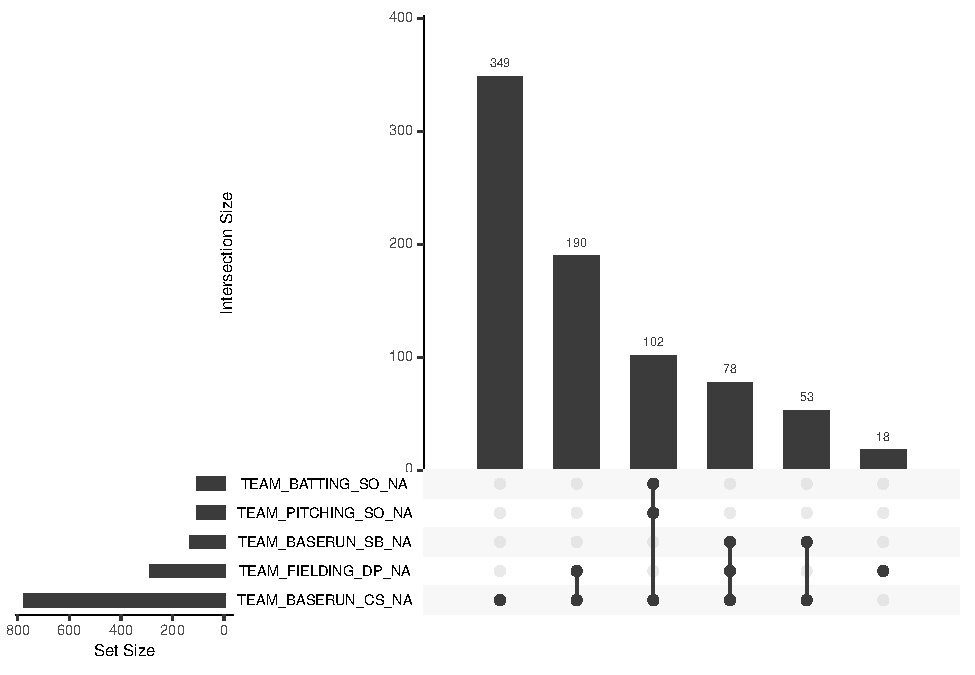
\includegraphics{Assignment1_files/figure-latex/unnamed-chunk-16-1.pdf}

\begin{Shaded}
\begin{Highlighting}[]
\FunctionTok{gg\_miss\_case}\NormalTok{(train\_data)}\SpecialCharTok{+}
  \FunctionTok{theme\_classic}\NormalTok{()}
\end{Highlighting}
\end{Shaded}

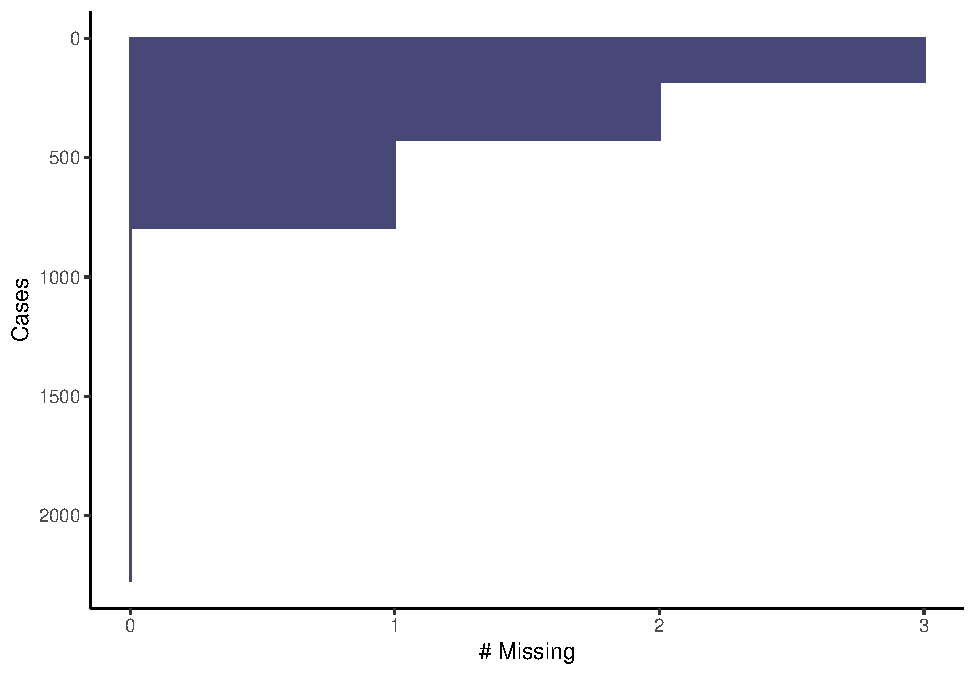
\includegraphics{Assignment1_files/figure-latex/unnamed-chunk-16-2.pdf}
By looking at the patterns and intersections of missing data among the
variables. We can see that 5 variables have missing values,
Team\_BATTING has the most missing values so we are completely removing
these observations. Overall, the pattern suggests that the variables are
Missing at Random (MAR).

When it comes to fixing missing values,there are several methods at our
disposal. The first technique is to fill the missing values with the
mean values of each variable. We'll use the Hmisc R Package to fill the
missing data with the mean, most of the time, mean imputation will lead
to good results. The same procedure will be used for the other variables
with missing values in Model 2 but by using the Median instead of the
mean

The second technique for imputing missing values is to use a decision
tree. This is slightly more involved, but will likely give the better
results. A decision tree will be created for each variable with missing
values. In mean imputation, a fixed value is used for missing values of
an entire variable whereas in decision tree imputation, a value is used
based on certain conditions.

\hypertarget{build-models}{%
\subsection{Build Models}\label{build-models}}

\hypertarget{model-1-mean-full-model}{%
\subsubsection{MODEL 1: MEAN FULL MODEL}\label{model-1-mean-full-model}}

This is a full model containing all the variables with the meanusred for
missing values. This is a good starting model to determine how well each
variable helps predict wins. The mean is generally an adequate guess for
missing values. In this model, no selection technique is used. All
variables are manually included.

To the that we used the Hmisc R package to imputes missing value using
user defined statistical method (mean in our case)

\begin{Shaded}
\begin{Highlighting}[]
\NormalTok{model1 }\OtherTok{\textless{}{-}} \FunctionTok{lm}\NormalTok{(TARGET\_WINS }\SpecialCharTok{\textasciitilde{}} 
\NormalTok{               TEAM\_BATTING\_H }\SpecialCharTok{+}   \CommentTok{\# Base Hits by batters (1B,2B,3B,HR)}
\NormalTok{               TEAM\_BATTING\_2B }\SpecialCharTok{+}  \CommentTok{\# Doubles by batters (2B) }
\NormalTok{               TEAM\_BATTING\_3B }\SpecialCharTok{+}  \CommentTok{\# Triples by batters (3B)}
\NormalTok{               TEAM\_BATTING\_HR }\SpecialCharTok{+}  \CommentTok{\# Homeruns by batters (4B) }
\NormalTok{               TEAM\_BATTING\_BB }\SpecialCharTok{+}  \CommentTok{\# Walks by batters}
\NormalTok{               TEAM\_BATTING\_SO }\SpecialCharTok{+}  \CommentTok{\# Strikeouts by batters }
\NormalTok{               TEAM\_BASERUN\_SB }\SpecialCharTok{+}  \CommentTok{\# Stolen bases}
\NormalTok{               TEAM\_BASERUN\_CS }\SpecialCharTok{+}  \CommentTok{\# Caught stealing }
\NormalTok{               TEAM\_PITCHING\_H }\SpecialCharTok{+}  \CommentTok{\# Hits allowed}
\NormalTok{               TEAM\_PITCHING\_HR }\SpecialCharTok{+} \CommentTok{\# Homeruns allowed}
\NormalTok{               TEAM\_PITCHING\_BB }\SpecialCharTok{+} \CommentTok{\# Walks allowed}
\NormalTok{               TEAM\_PITCHING\_SO }\SpecialCharTok{+} \CommentTok{\# Strikeouts by pitchers}
\NormalTok{               TEAM\_FIELDING\_E }\SpecialCharTok{+}  \CommentTok{\# Errors}
\NormalTok{               TEAM\_FIELDING\_DP,  }\CommentTok{\# Double Plays}
             \AttributeTok{data=}\NormalTok{train\_model1)}
\FunctionTok{summary}\NormalTok{(model1)}
\end{Highlighting}
\end{Shaded}

\begin{verbatim}
## 
## Call:
## lm(formula = TARGET_WINS ~ TEAM_BATTING_H + TEAM_BATTING_2B + 
##     TEAM_BATTING_3B + TEAM_BATTING_HR + TEAM_BATTING_BB + TEAM_BATTING_SO + 
##     TEAM_BASERUN_SB + TEAM_BASERUN_CS + TEAM_PITCHING_H + TEAM_PITCHING_HR + 
##     TEAM_PITCHING_BB + TEAM_PITCHING_SO + TEAM_FIELDING_E + TEAM_FIELDING_DP, 
##     data = train_model1)
## 
## Residuals:
##     Min      1Q  Median      3Q     Max 
## -35.113  -7.633  -0.018   7.324  45.214 
## 
## Coefficients:
##                   Estimate Std. Error t value Pr(>|t|)    
## (Intercept)      59.237509   6.113895   9.689  < 2e-16 ***
## TEAM_BATTING_H   -0.002070   0.005441  -0.380 0.703633    
## TEAM_BATTING_2B  -0.023765   0.008808  -2.698 0.007034 ** 
## TEAM_BATTING_3B   0.168568   0.018723   9.003  < 2e-16 ***
## TEAM_BATTING_HR   0.321816   0.055324   5.817 6.98e-09 ***
## TEAM_BATTING_BB   0.093055   0.018164   5.123 3.30e-07 ***
## TEAM_BATTING_SO  -0.049966   0.008917  -5.603 2.40e-08 ***
## TEAM_BASERUN_SB   0.081187   0.006161  13.178  < 2e-16 ***
## TEAM_BASERUN_CS  -0.059350   0.014616  -4.061 5.09e-05 ***
## TEAM_PITCHING_H   0.025458   0.002263  11.251  < 2e-16 ***
## TEAM_PITCHING_HR -0.216833   0.052137  -4.159 3.33e-05 ***
## TEAM_PITCHING_BB -0.060526   0.016914  -3.578 0.000354 ***
## TEAM_PITCHING_SO  0.028051   0.007993   3.509 0.000459 ***
## TEAM_FIELDING_E  -0.084678   0.005292 -16.001  < 2e-16 ***
## TEAM_FIELDING_DP -0.120255   0.012485  -9.632  < 2e-16 ***
## ---
## Signif. codes:  0 '***' 0.001 '**' 0.01 '*' 0.05 '.' 0.1 ' ' 1
## 
## Residual standard error: 10.96 on 1975 degrees of freedom
##   (286 observations deleted due to missingness)
## Multiple R-squared:  0.3858, Adjusted R-squared:  0.3814 
## F-statistic: 88.61 on 14 and 1975 DF,  p-value: < 2.2e-16
\end{verbatim}

Mean Square Error (MSE)

\begin{Shaded}
\begin{Highlighting}[]
\FunctionTok{mean}\NormalTok{(model1}\SpecialCharTok{$}\NormalTok{residuals}\SpecialCharTok{\^{}}\DecValTok{2}\NormalTok{)}
\end{Highlighting}
\end{Shaded}

\begin{verbatim}
## [1] 119.3236
\end{verbatim}

\begin{Shaded}
\begin{Highlighting}[]
\FunctionTok{layout}\NormalTok{(}\FunctionTok{matrix}\NormalTok{(}\FunctionTok{c}\NormalTok{(}\DecValTok{1}\NormalTok{,}\DecValTok{2}\NormalTok{,}\DecValTok{3}\NormalTok{,}\DecValTok{4}\NormalTok{),}\DecValTok{2}\NormalTok{,}\DecValTok{2}\NormalTok{)) }\CommentTok{\# optional 4 graphs/page}
\FunctionTok{plot}\NormalTok{(model1)}
\end{Highlighting}
\end{Shaded}

\includegraphics{Assignment1_files/figure-latex/unnamed-chunk-20-1.pdf}

The overall p-value for Model 1is less than 0.0001,which indicates a
significant model in predicting wins. The Adjusted R-Squared and Mean
Square Error (MSE) will be the metrics used to determine the best
model.A higher Adjusted R-Squared is better and a lower MSE is better.In
this case, the Adjusted R-Squared is 0.3814 and MSE is 168.91, which
will be the current benchmark.

\textbf{The resulting equation for Model 1 is :}

\begin{center}

WINS =+ 25.06831 \\
      +0.0473146*Base Hits by batters \\
      -0.0209806*Doubles by batters \\
      +0.0692224*Triples by batters \\
      +0.0680963*Homeruns by batters \\
      +0.0108690*Walks by batters \\
      -0.0081244*Strikeouts by batters \\
      +0.0299345*Stolen bases \\
      -0.01173*Caught stealing \\
      -0.00073149*Hits allowed \\
      +0.01481*Homeruns allowed \\
      +0.00008066*Walks allowed \\
      +0.0026600*Strikeouts by pitchers \\
      -0.02118*Errors \\
      -0.1208451*Double plays \\
\end{center}

Most of Model 1 makes senseas positive measures of success like Base
Hits, Triples, Homeruns, Walks by batters, and Stolen bases are positive
coefficients in the equation while negative measures of success like
Strikeouts by batters, Caught stealing, Hits allowed, and Errors are
negative coefficients in the equation.All these values make intuitive
sense.On the other hand, Doubles and Double plays are shown as negative
coefficients when they should have a positive impact on wins. Also,
Homeruns allowed and Walks allowed are shown as positive coefficients
when they should have negative impact on wins.These values are counter
intuitive.The counter intuitive parts of the model may need to be
further investigated if this model were to be chosen for
deployment.However, for now, the model will be kept as a benchmark
despite certain measures not making sense.

\hypertarget{model-2-median-with-stepwise}{%
\subsubsection{MODEL 2: MEDIAN WITH
STEPWISE}\label{model-2-median-with-stepwise}}

Earlier in the exploration of the data, the analysis revealed the
possibility of outliers present in the data. Because the mean is highly
influenced by outliers, this model attempts to remedy that by using the
median to impute missing values.Model 2 is a significant model based on
the p-value of less than 0.0001. The Adjusted R-Squared is 0.3147 and
MSE is 169.799.

\begin{Shaded}
\begin{Highlighting}[]
\NormalTok{train\_model2 }\OtherTok{\textless{}{-}}\NormalTok{ train\_data}
\CommentTok{\# Filling missing values with Mean using the impute package}
\NormalTok{train\_model2}\SpecialCharTok{$}\NormalTok{TEAM\_BATTING\_SO[}\FunctionTok{is.na}\NormalTok{(train\_model2}\SpecialCharTok{$}\NormalTok{TEAM\_BATTING\_SO)] }\OtherTok{=} \FunctionTok{median}\NormalTok{(train\_model2}\SpecialCharTok{$}\NormalTok{TEAM\_BATTING\_SO, }\AttributeTok{na.rm=}\ConstantTok{TRUE}\NormalTok{)}
\NormalTok{train\_model2}\SpecialCharTok{$}\NormalTok{TEAM\_BASERUN\_SB[}\FunctionTok{is.na}\NormalTok{(train\_model2}\SpecialCharTok{$}\NormalTok{TEAM\_BASERUN\_SB)] }\OtherTok{=} \FunctionTok{median}\NormalTok{(train\_model2}\SpecialCharTok{$}\NormalTok{TEAM\_BASERUN\_SB, }\AttributeTok{na.rm=}\ConstantTok{TRUE}\NormalTok{)}
\NormalTok{train\_model2}\SpecialCharTok{$}\NormalTok{TEAM\_BASERUN\_CS[}\FunctionTok{is.na}\NormalTok{(train\_model2}\SpecialCharTok{$}\NormalTok{TEAM\_BASERUN\_CS)] }\OtherTok{=} \FunctionTok{median}\NormalTok{(train\_model2}\SpecialCharTok{$}\NormalTok{TEAM\_BASERUN\_CS, }\AttributeTok{na.rm=}\ConstantTok{TRUE}\NormalTok{)}
\NormalTok{train\_model2}\SpecialCharTok{$}\NormalTok{TEAM\_PITCHING\_SO[}\FunctionTok{is.na}\NormalTok{(train\_model2}\SpecialCharTok{$}\NormalTok{TEAM\_PITCHING\_SO)] }\OtherTok{=} \FunctionTok{median}\NormalTok{(train\_model2}\SpecialCharTok{$}\NormalTok{TEAM\_PITCHING\_SO, }\AttributeTok{na.rm=}\ConstantTok{TRUE}\NormalTok{)}
\CommentTok{\#train\_model2$TEAM\_FIELDING\_DP[is.na(train\_model2$TEAM\_FIELDING\_DP)] = median(train\_model2$TEAM\_FIELDING\_DP, na.rm=TRUE)}
\end{Highlighting}
\end{Shaded}

\begin{Shaded}
\begin{Highlighting}[]
\NormalTok{model2 }\OtherTok{\textless{}{-}} \FunctionTok{lm}\NormalTok{(TARGET\_WINS }\SpecialCharTok{\textasciitilde{}} 
\NormalTok{               TEAM\_BATTING\_H }\SpecialCharTok{+}   \CommentTok{\# Base Hits by batters (1B,2B,3B,HR)}
\NormalTok{               TEAM\_BATTING\_2B }\SpecialCharTok{+}  \CommentTok{\# Doubles by batters (2B) }
\NormalTok{               TEAM\_BATTING\_3B }\SpecialCharTok{+}  \CommentTok{\# Triples by batters (3B)}
\NormalTok{               TEAM\_BATTING\_HR }\SpecialCharTok{+}  \CommentTok{\# Homeruns by batters (4B) }
\NormalTok{               TEAM\_BATTING\_BB }\SpecialCharTok{+}  \CommentTok{\# Walks by batters}
\NormalTok{               TEAM\_BATTING\_SO }\SpecialCharTok{+}  \CommentTok{\# Strikeouts by batters }
\NormalTok{               TEAM\_BASERUN\_SB }\SpecialCharTok{+}  \CommentTok{\# Stolen bases}
\NormalTok{               TEAM\_BASERUN\_CS }\SpecialCharTok{+}  \CommentTok{\# Caught stealing }
\NormalTok{               TEAM\_PITCHING\_H }\SpecialCharTok{+}  \CommentTok{\# Hits allowed}
\NormalTok{               TEAM\_PITCHING\_HR }\SpecialCharTok{+} \CommentTok{\# Homeruns allowed}
\NormalTok{               TEAM\_PITCHING\_BB }\SpecialCharTok{+} \CommentTok{\# Walks allowed}
\NormalTok{               TEAM\_PITCHING\_SO }\SpecialCharTok{+} \CommentTok{\# Strikeouts by pitchers}
\NormalTok{               TEAM\_FIELDING\_E }\SpecialCharTok{+}  \CommentTok{\# Errors}
\NormalTok{               TEAM\_FIELDING\_DP,  }\CommentTok{\# Double Plays}
             \AttributeTok{data=}\NormalTok{train\_model2)}
\FunctionTok{summary}\NormalTok{(model1)}
\end{Highlighting}
\end{Shaded}

\begin{verbatim}
## 
## Call:
## lm(formula = TARGET_WINS ~ TEAM_BATTING_H + TEAM_BATTING_2B + 
##     TEAM_BATTING_3B + TEAM_BATTING_HR + TEAM_BATTING_BB + TEAM_BATTING_SO + 
##     TEAM_BASERUN_SB + TEAM_BASERUN_CS + TEAM_PITCHING_H + TEAM_PITCHING_HR + 
##     TEAM_PITCHING_BB + TEAM_PITCHING_SO + TEAM_FIELDING_E + TEAM_FIELDING_DP, 
##     data = train_model1)
## 
## Residuals:
##     Min      1Q  Median      3Q     Max 
## -35.113  -7.633  -0.018   7.324  45.214 
## 
## Coefficients:
##                   Estimate Std. Error t value Pr(>|t|)    
## (Intercept)      59.237509   6.113895   9.689  < 2e-16 ***
## TEAM_BATTING_H   -0.002070   0.005441  -0.380 0.703633    
## TEAM_BATTING_2B  -0.023765   0.008808  -2.698 0.007034 ** 
## TEAM_BATTING_3B   0.168568   0.018723   9.003  < 2e-16 ***
## TEAM_BATTING_HR   0.321816   0.055324   5.817 6.98e-09 ***
## TEAM_BATTING_BB   0.093055   0.018164   5.123 3.30e-07 ***
## TEAM_BATTING_SO  -0.049966   0.008917  -5.603 2.40e-08 ***
## TEAM_BASERUN_SB   0.081187   0.006161  13.178  < 2e-16 ***
## TEAM_BASERUN_CS  -0.059350   0.014616  -4.061 5.09e-05 ***
## TEAM_PITCHING_H   0.025458   0.002263  11.251  < 2e-16 ***
## TEAM_PITCHING_HR -0.216833   0.052137  -4.159 3.33e-05 ***
## TEAM_PITCHING_BB -0.060526   0.016914  -3.578 0.000354 ***
## TEAM_PITCHING_SO  0.028051   0.007993   3.509 0.000459 ***
## TEAM_FIELDING_E  -0.084678   0.005292 -16.001  < 2e-16 ***
## TEAM_FIELDING_DP -0.120255   0.012485  -9.632  < 2e-16 ***
## ---
## Signif. codes:  0 '***' 0.001 '**' 0.01 '*' 0.05 '.' 0.1 ' ' 1
## 
## Residual standard error: 10.96 on 1975 degrees of freedom
##   (286 observations deleted due to missingness)
## Multiple R-squared:  0.3858, Adjusted R-squared:  0.3814 
## F-statistic: 88.61 on 14 and 1975 DF,  p-value: < 2.2e-16
\end{verbatim}

\begin{Shaded}
\begin{Highlighting}[]
\FunctionTok{mean}\NormalTok{(model2}\SpecialCharTok{$}\NormalTok{residuals}\SpecialCharTok{\^{}}\DecValTok{2}\NormalTok{)}
\end{Highlighting}
\end{Shaded}

\begin{verbatim}
## [1] 120.1388
\end{verbatim}

\begin{Shaded}
\begin{Highlighting}[]
\FunctionTok{layout}\NormalTok{(}\FunctionTok{matrix}\NormalTok{(}\FunctionTok{c}\NormalTok{(}\DecValTok{1}\NormalTok{,}\DecValTok{2}\NormalTok{,}\DecValTok{3}\NormalTok{,}\DecValTok{4}\NormalTok{),}\DecValTok{2}\NormalTok{,}\DecValTok{2}\NormalTok{)) }\CommentTok{\# optional 4 graphs/page}
\FunctionTok{plot}\NormalTok{(model2)}
\end{Highlighting}
\end{Shaded}

\includegraphics{Assignment1_files/figure-latex/unnamed-chunk-24-1.pdf}

\textbf{The resulting equation for Model 2 is :}

\begin{center}

WINS =+ 25.0602 \\
      +0.04824*Base Hits by batters \\
      -0.02006*Doubles by batters \\
      +0.06047*Triples by batters \\
      +0.05299*Homeruns by batters \\
      +0.01042*Walks by batters \\
      -0.009349*Strikeouts by batters \\
      +0.02949*Stolen bases \\
      -0.01188*Caught stealing \\
      -0.0007342*Hits allowed \\
      +0.01480*Homeruns allowed \\
      +0.00008891*Walks allowed \\
      +0.002843*Strikeouts by pitchers \\
      -0.02112*Errors \\
      -0.1210*Double plays \\
\end{center}

\hypertarget{model-3-decision-tree}{%
\subsubsection{MODEL 3: Decision Tree}\label{model-3-decision-tree}}

Decision trees are extremely useful in fixing missing values. In Model
3, a decision tree will be used. The missing values will be filled in
based on conditions of other variables. Decision trees can provide more
accurate guesses which can produce more accurate models.Stepwise
variable selection will be used again because of its ability to add and
remove variables at each iteration.

\begin{Shaded}
\begin{Highlighting}[]
\FunctionTok{library}\NormalTok{(rpart)}
\NormalTok{train\_model3 }\OtherTok{\textless{}{-}}\NormalTok{train\_data[,}\SpecialCharTok{{-}}\FunctionTok{c}\NormalTok{(}\DecValTok{1}\NormalTok{)]}
\FunctionTok{names}\NormalTok{(train\_model3)}
\end{Highlighting}
\end{Shaded}

\begin{verbatim}
##  [1] "TARGET_WINS"      "TEAM_BATTING_H"   "TEAM_BATTING_2B"  "TEAM_BATTING_3B" 
##  [5] "TEAM_BATTING_HR"  "TEAM_BATTING_BB"  "TEAM_BATTING_SO"  "TEAM_BASERUN_SB" 
##  [9] "TEAM_BASERUN_CS"  "TEAM_PITCHING_H"  "TEAM_PITCHING_HR" "TEAM_PITCHING_BB"
## [13] "TEAM_PITCHING_SO" "TEAM_FIELDING_E"  "TEAM_FIELDING_DP" "TEAM_BATTING_SLG"
\end{verbatim}

create a decision tree for each variable with missing values. cross
validate to see if we can prune the tree to make simpler\#
TEAM\_BATTING\_SO, TEAM\_BASERUN\_CS, TEAM\_BASERUN\_SB,
TEAM\_PITCHING\_SO, TEAM\_FIELDING\_DP

\begin{Shaded}
\begin{Highlighting}[]
\NormalTok{batting\_so\_tree }\OtherTok{\textless{}{-}}\FunctionTok{rpart}\NormalTok{(TEAM\_BATTING\_SO}\SpecialCharTok{\textasciitilde{}}\NormalTok{.,}\AttributeTok{data=}\NormalTok{train\_model3)}
\FunctionTok{plot}\NormalTok{(batting\_so\_tree)}
\FunctionTok{text}\NormalTok{(batting\_so\_tree)}
\end{Highlighting}
\end{Shaded}

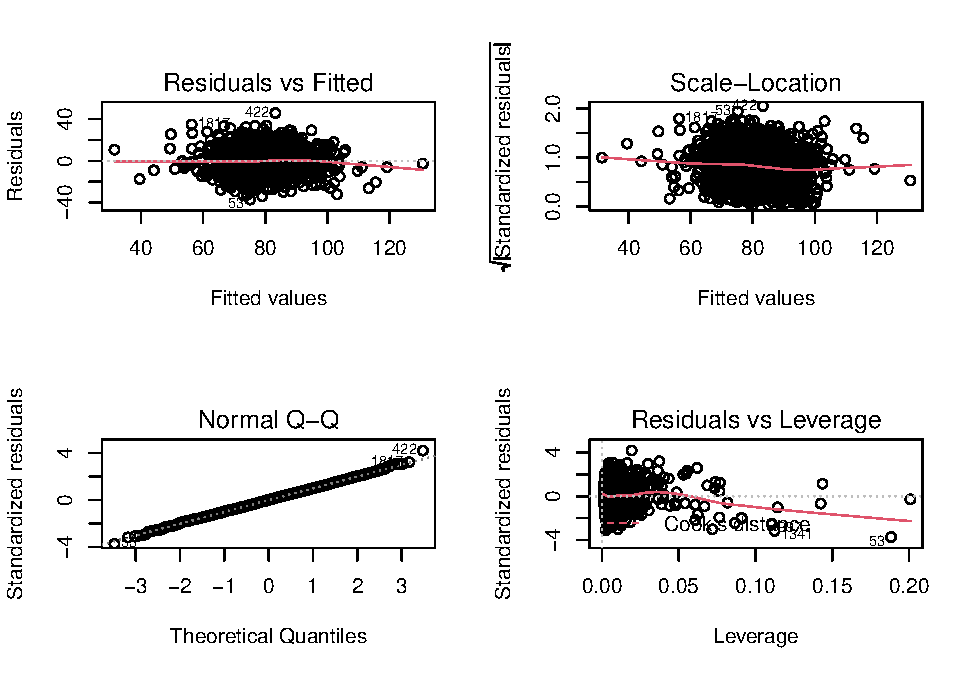
\includegraphics{Assignment1_files/figure-latex/unnamed-chunk-26-1.pdf}

\begin{Shaded}
\begin{Highlighting}[]
\FunctionTok{printcp}\NormalTok{(batting\_so\_tree)}
\end{Highlighting}
\end{Shaded}

\begin{verbatim}
## 
## Regression tree:
## rpart(formula = TEAM_BATTING_SO ~ ., data = train_model3)
## 
## Variables actually used in tree construction:
## [1] TEAM_FIELDING_E  TEAM_PITCHING_H  TEAM_PITCHING_SO
## 
## Root node error: 134216171/2174 = 61737
## 
## n=2174 (102 observations deleted due to missingness)
## 
##         CP nsplit rel error  xerror      xstd
## 1 0.599100      0   1.00000 1.00073 0.0278413
## 2 0.085676      1   0.40090 0.40828 0.0187247
## 3 0.083615      2   0.31522 0.35671 0.0175075
## 4 0.056843      3   0.23161 0.23945 0.0107212
## 5 0.038679      4   0.17477 0.18314 0.0104590
## 6 0.016972      5   0.13609 0.14812 0.0090572
## 7 0.012470      6   0.11912 0.12802 0.0078935
## 8 0.010000      7   0.10665 0.12071 0.0081424
\end{verbatim}

\begin{Shaded}
\begin{Highlighting}[]
\FunctionTok{plotcp}\NormalTok{(batting\_so\_tree) }\CommentTok{\# keep all 8 branches}
\end{Highlighting}
\end{Shaded}

\includegraphics{Assignment1_files/figure-latex/unnamed-chunk-26-2.pdf}

\begin{Shaded}
\begin{Highlighting}[]
\NormalTok{baserun\_cs }\OtherTok{\textless{}{-}}\FunctionTok{rpart}\NormalTok{(TEAM\_BASERUN\_CS}\SpecialCharTok{\textasciitilde{}}\NormalTok{.,}\AttributeTok{data=}\NormalTok{train\_model3)}
\FunctionTok{plot}\NormalTok{(baserun\_cs)}
\FunctionTok{text}\NormalTok{(baserun\_cs)}
\end{Highlighting}
\end{Shaded}

\includegraphics{Assignment1_files/figure-latex/unnamed-chunk-27-1.pdf}

\begin{Shaded}
\begin{Highlighting}[]
\FunctionTok{printcp}\NormalTok{(baserun\_cs)}
\end{Highlighting}
\end{Shaded}

\begin{verbatim}
## 
## Regression tree:
## rpart(formula = TEAM_BASERUN_CS ~ ., data = train_model3)
## 
## Variables actually used in tree construction:
## [1] TEAM_BASERUN_SB  TEAM_BATTING_HR  TEAM_FIELDING_E  TEAM_PITCHING_HR
## [5] TEAM_PITCHING_SO
## 
## Root node error: 792071/1504 = 526.64
## 
## n=1504 (772 observations deleted due to missingness)
## 
##          CP nsplit rel error  xerror     xstd
## 1  0.250637      0   1.00000 1.00125 0.080210
## 2  0.177503      1   0.74936 0.78248 0.062274
## 3  0.073198      2   0.57186 0.62840 0.035395
## 4  0.040757      3   0.49866 0.55771 0.032512
## 5  0.030634      4   0.45790 0.53738 0.031253
## 6  0.027470      5   0.42727 0.49988 0.028894
## 7  0.017752      6   0.39980 0.47379 0.026566
## 8  0.015197      7   0.38205 0.45661 0.025951
## 9  0.010628      8   0.36685 0.44300 0.026495
## 10 0.010000      9   0.35622 0.43767 0.025319
\end{verbatim}

\begin{Shaded}
\begin{Highlighting}[]
\FunctionTok{plotcp}\NormalTok{(baserun\_cs) }\CommentTok{\# keep all 10 branches}
\end{Highlighting}
\end{Shaded}

\includegraphics{Assignment1_files/figure-latex/unnamed-chunk-27-2.pdf}

\begin{Shaded}
\begin{Highlighting}[]
\NormalTok{baserun\_sb }\OtherTok{\textless{}{-}}\FunctionTok{rpart}\NormalTok{(TEAM\_BASERUN\_SB}\SpecialCharTok{\textasciitilde{}}\NormalTok{.,}\AttributeTok{data=}\NormalTok{train\_model3)}
\FunctionTok{plot}\NormalTok{(baserun\_sb)}
\FunctionTok{text}\NormalTok{(baserun\_sb)}
\end{Highlighting}
\end{Shaded}

\includegraphics{Assignment1_files/figure-latex/unnamed-chunk-28-1.pdf}

\begin{Shaded}
\begin{Highlighting}[]
\FunctionTok{printcp}\NormalTok{(baserun\_sb)}
\end{Highlighting}
\end{Shaded}

\begin{verbatim}
## 
## Regression tree:
## rpart(formula = TEAM_BASERUN_SB ~ ., data = train_model3)
## 
## Variables actually used in tree construction:
## [1] TARGET_WINS      TEAM_BASERUN_CS  TEAM_BATTING_HR  TEAM_BATTING_SLG
## [5] TEAM_BATTING_SO  TEAM_FIELDING_E  TEAM_PITCHING_BB
## 
## Root node error: 16524427/2145 = 7703.7
## 
## n=2145 (131 observations deleted due to missingness)
## 
##          CP nsplit rel error  xerror     xstd
## 1  0.462843      0   1.00000 1.00110 0.059208
## 2  0.069582      1   0.53716 0.54188 0.031304
## 3  0.049303      2   0.46758 0.48076 0.027890
## 4  0.027398      3   0.41827 0.43347 0.027518
## 5  0.017095      5   0.36348 0.39084 0.023232
## 6  0.015940      7   0.32929 0.37973 0.024696
## 7  0.012535      8   0.31335 0.37497 0.024615
## 8  0.011580      9   0.30081 0.35070 0.021859
## 9  0.010267     10   0.28923 0.34593 0.021781
## 10 0.010000     11   0.27896 0.34601 0.021607
\end{verbatim}

\begin{Shaded}
\begin{Highlighting}[]
\FunctionTok{plotcp}\NormalTok{(baserun\_sb) }\CommentTok{\# keep all 10 branches (maybe 8)}
\end{Highlighting}
\end{Shaded}

\includegraphics{Assignment1_files/figure-latex/unnamed-chunk-28-2.pdf}

\begin{Shaded}
\begin{Highlighting}[]
\NormalTok{pitching\_so }\OtherTok{\textless{}{-}}\FunctionTok{rpart}\NormalTok{(TEAM\_PITCHING\_SO}\SpecialCharTok{\textasciitilde{}}\NormalTok{.,}\AttributeTok{data=}\NormalTok{train\_model3)}
\FunctionTok{plot}\NormalTok{(pitching\_so)}
\FunctionTok{text}\NormalTok{(pitching\_so)}
\end{Highlighting}
\end{Shaded}

\includegraphics{Assignment1_files/figure-latex/unnamed-chunk-29-1.pdf}

\begin{Shaded}
\begin{Highlighting}[]
\FunctionTok{printcp}\NormalTok{(pitching\_so)}
\end{Highlighting}
\end{Shaded}

\begin{verbatim}
## 
## Regression tree:
## rpart(formula = TEAM_PITCHING_SO ~ ., data = train_model3)
## 
## Variables actually used in tree construction:
## [1] TEAM_BATTING_SO  TEAM_FIELDING_E  TEAM_PITCHING_BB
## 
## Root node error: 664727332/2174 = 305762
## 
## n=2174 (102 observations deleted due to missingness)
## 
##         CP nsplit rel error  xerror    xstd
## 1 0.248066      0   1.00000 1.00093 0.55711
## 2 0.112677      1   0.75193 0.96827 0.52405
## 3 0.037586      2   0.63926 0.67885 0.34327
## 4 0.016286      3   0.60167 0.67212 0.34325
## 5 0.014874      4   0.58538 0.65783 0.34332
## 6 0.010000      5   0.57051 0.64179 0.34333
\end{verbatim}

\begin{Shaded}
\begin{Highlighting}[]
\FunctionTok{plotcp}\NormalTok{(pitching\_so) }\CommentTok{\# keep all 6 branches (maybe 5)}
\end{Highlighting}
\end{Shaded}

\includegraphics{Assignment1_files/figure-latex/unnamed-chunk-29-2.pdf}

\begin{Shaded}
\begin{Highlighting}[]
\NormalTok{fielding\_dp }\OtherTok{\textless{}{-}}\FunctionTok{rpart}\NormalTok{(TEAM\_FIELDING\_DP}\SpecialCharTok{\textasciitilde{}}\NormalTok{.,}\AttributeTok{data=}\NormalTok{train\_model3)}
\FunctionTok{plot}\NormalTok{(fielding\_dp)}
\FunctionTok{text}\NormalTok{(fielding\_dp)}
\end{Highlighting}
\end{Shaded}

\includegraphics{Assignment1_files/figure-latex/unnamed-chunk-30-1.pdf}

\begin{Shaded}
\begin{Highlighting}[]
\FunctionTok{printcp}\NormalTok{(fielding\_dp)}
\end{Highlighting}
\end{Shaded}

\begin{verbatim}
## 
## Regression tree:
## rpart(formula = TEAM_FIELDING_DP ~ ., data = train_model3)
## 
## Variables actually used in tree construction:
## [1] TEAM_BASERUN_SB TEAM_BATTING_HR TEAM_BATTING_SO TEAM_FIELDING_E
## 
## Root node error: 1368081/1990 = 687.48
## 
## n=1990 (286 observations deleted due to missingness)
## 
##         CP nsplit rel error  xerror     xstd
## 1 0.358546      0   1.00000 1.00157 0.033177
## 2 0.035856      1   0.64145 0.65933 0.022702
## 3 0.027639      2   0.60560 0.62564 0.021098
## 4 0.017750      3   0.57796 0.60379 0.020000
## 5 0.011065      4   0.56021 0.58509 0.019264
## 6 0.010000      6   0.53808 0.57970 0.019093
\end{verbatim}

\begin{Shaded}
\begin{Highlighting}[]
\FunctionTok{plotcp}\NormalTok{(fielding\_dp) }\CommentTok{\# keep all 6 branches}
\end{Highlighting}
\end{Shaded}

\includegraphics{Assignment1_files/figure-latex/unnamed-chunk-30-2.pdf}
Behind the scenes rpart is automatically applying a range of cost
complexity (α values to prune the tree. To compare the error for each α
value, rpart performs a 10-fold cross validation so that the error
associated with a given α value is computed on the hold-out validation
data.

The complexity parameter (cp) in rpart is the minimum improvement in the
model needed at each node. It's based on the cost complexity of the
model defined as

The cp value is a stopping parameter. It helps speed up the search for
splits because it can identify splits that don't meet this criteria and
prune them before going too far.

Now lets run the model

\hypertarget{select-a-model}{%
\subsection{Select A Model}\label{select-a-model}}

\hypertarget{appendix}{%
\subsection{Appendix}\label{appendix}}

\hypertarget{references}{%
\subsection{References}\label{references}}

\textless\textless\textless\textless\textless\textless\textless{} HEAD

\begin{itemize}
\item
  Dealing with Missing Data using R :
  \url{https://medium.com/coinmonks/dealing-with-missing-data-using-r-3ae428da2d17}
\item
  Decision Tree :
  \url{http://www.learnbymarketing.com/tutorials/rpart-decision-trees-in-r/}
\item
  Decision Tree :
  \url{https://www.datacamp.com/community/tutorials/decision-trees-R}
\item ~
  \hypertarget{introduction-to-data-science-case-study-moneyball-httpsrafalab.github.iodsbooklinear-models.htmlcase-study-moneyball}{%
  \section{\texorpdfstring{Introduction to Data Science (Case Study
  Moneyball):
  \url{https://rafalab.github.io/dsbook/linear-models.html\#case-study-moneyball}}{Introduction to Data Science (Case Study Moneyball): https://rafalab.github.io/dsbook/linear-models.html\#case-study-moneyball}}\label{introduction-to-data-science-case-study-moneyball-httpsrafalab.github.iodsbooklinear-models.htmlcase-study-moneyball}}

  \begin{quote}
  \begin{quote}
  \begin{quote}
  \begin{quote}
  \begin{quote}
  \begin{quote}
  \begin{quote}
  bf59d52d90d6b4ab9b840f4b7fa1cd132debf1fb
  \end{quote}
  \end{quote}
  \end{quote}
  \end{quote}
  \end{quote}
  \end{quote}
  \end{quote}
\end{itemize}

\end{document}
